% Preambel (utenfor ankersjekken: bare oppsett, ingen påstander)
\documentclass[11pt,a4paper]{article}
\usepackage[T1]{fontenc}
\usepackage[utf8]{inputenc}
\usepackage{lmodern}
\usepackage[margin=2.5cm]{geometry}
\usepackage{microtype}
\usepackage{booktabs}
\usepackage{graphicx}
\usepackage{amsmath}
\usepackage{caption}
\usepackage[hidelinks]{hyperref}
\makeatletter\g@addto@macro\UrlBreaks{\do\_}\makeatother
\captionsetup{font=small,labelfont=bf}
\newcommand{\figbredde}{0.98\linewidth}
% generert av tools/lag_manus.py fra resultater/utfall.csv sha256 0b44f987e967e11133af9527bd3b88843689661e4add3e3314686f67ee287b13 [GT-647]; resultater/h_under_null.csv sha256 204cdbca68e3a99eea6e7e40649465cddd1e3c24253329a3f213942d1083d596 [GT-648]
\newcommand{\resGyldigeTimerPrimaer}{17567}
\newcommand{\resTimerIRutenett}{17568}
\newcommand{\resManglendeTimerPrimaer}{1}
\newcommand{\resPrimFullNOone}{1015}
\newcommand{\resPrimHalfNOone}{120}
\newcommand{\resSekFullNOone}{180}
\newcommand{\resSekGyldigeNOone}{17567}
\newcommand{\resHnegNOone}{0}
\newcommand{\resHnegFoerNOone}{0}
\newcommand{\resPrimFullNOtwo}{1424}
\newcommand{\resPrimHalfNOtwo}{85}
\newcommand{\resSekFullNOtwo}{0}
\newcommand{\resSekGyldigeNOtwo}{16717}
\newcommand{\resHnegNOtwo}{0}
\newcommand{\resHnegFoerNOtwo}{0}
\newcommand{\resPrimFullNOthree}{1333}
\newcommand{\resPrimHalfNOthree}{285}
\newcommand{\resSekFullNOthree}{0}
\newcommand{\resSekGyldigeNOthree}{16919}
\newcommand{\resHnegNOthree}{0}
\newcommand{\resHnegFoerNOthree}{0}
\newcommand{\resPrimFullNOfour}{4984}
\newcommand{\resPrimHalfNOfour}{702}
\newcommand{\resSekFullNOfour}{0}
\newcommand{\resSekGyldigeNOfour}{17567}
\newcommand{\resHnegNOfour}{0}
\newcommand{\resHnegFoerNOfour}{0}
\newcommand{\resPrimFullNOfive}{53}
\newcommand{\resPrimHalfNOfive}{23}
\newcommand{\resSekFullNOfive}{0}
\newcommand{\resSekGyldigeNOfive}{17281}
\newcommand{\resHnegNOfive}{8}
\newcommand{\resHnegFoerNOfive}{8}
\newcommand{\resPrimNullFoer}{8}


\begin{document}

\title{Data-centre queues against flow-based import limits in the Norwegian bidding zones: a preregistered descriptive analysis}
\author{Eirik Botten Nicolaysen\\EcoDeco AS}
\date{}
\maketitle

\begin{abstract}
\noindent
We ask in how many market time units the data-centre queue in a Norwegian bidding zone, added as load in that zone, would require more import than the published minimum net position allows. % GT-179
The headroom is the realised day-ahead net position minus the minimum net position from the Nordic flow-based capacity calculation, adapted from the import-headroom definition of Xu and Stiewe~\cite{xu}: we use the signed difference NP $-$ minNP and keep negative values, where Xu and Stiewe use the absolute difference. % GT-182 GT-192 GT-357 GT-073
The analysis covers 2024-10-30 to 2026-10-31 for the five Norwegian zones and the share $f$ of the queue on a grid of 101 points. % GT-180 GT-201
A secondary measure adds the regulable hydropower that was not producing, and is an optimistic upper bound. % GT-183 GT-350
Methods were preregistered in a signed git tag and submitted to OSF Registries before any outcome was computed~\cite{osf}; three deviations are reported. % GT-437 GT-753
At $f = 1.00$ in the primary scenario, the number of hours with an event over the whole period ranges from \resPrimFullNOfive{} (NO5) to \resPrimFullNOfour{} (NO4) for the primary measure, out of \resGyldigeTimerPrimaer{} valid hours. % GT-196
The results are descriptive; they make no claim about actual security of supply, prices or connection capacity.
\end{abstract}

\section{Introduction}
\label{sec:intro}

On 09.11.2026 Statnett announced: ``Statnett innfører en midlertidig stans av ytterligere reservasjon av nettkapasitet til datasentre'' (Statnett is introducing a temporary halt to further reservation of grid capacity for data centres)~\cite{press}. % GT-679 GT-680
The halt concerns further reservation of grid capacity; according to Statnett, the decision does not mean a general halt in connecting data centres, and existing connections are not affected~\cite{press}. Statnett gives the systemic properties of data centres as the reason~\cite{press}. % GT-679 GT-775 GT-776 GT-037
Statnett reports the data-centre queue per Norwegian bidding zone as reserved capacity and capacity queue~\cite{pbi}. % GT-016 GT-017 GT-395
The question we ask is the one in the preregistration~\cite{osf}: the share of market time units (MTUs) in which the data-centre queue, added as load in the zone, would require more import than the minimum net position allows, per Norwegian bidding zone, as a function of the share $f$ of the queue that is added. % GT-179

Our earlier analysis, KHEPRI-DC v1~\cite{v1}, added the queue as flat load to observed production minus load, but did not test import. % GT-012 GT-031
Its interpretation rules treated import as normal operation without testing any limit~\cite{v1}. % GT-032 GT-033

\paragraph{Positioning.}
No page in our source archive as it stood after the first source reading (K-01--K-33; all sources are listed with URL, retrieval time and sha256 in the supplement \texttt{sources.csv}~\cite{sources}) has data-centre terms and net-position terms together, apart from v1's own files. % GT-135
The closest are:
\begin{itemize}
\item Statnett's reply to NVE~\cite{statnettbrev}, which uses a fixed realised import capacity into the Northern area of 1050 MW and does not use flow-based terms; % GT-130 GT-133
\item Xu and Stiewe~\cite{xu}, who define the import headroom but use data ``only published for the Core FBMC region'' and have no Nordic zones; % GT-077 GT-079
\item KHEPRI-DC v1~\cite{v1}, which does not test import. % GT-031
\end{itemize}
We do not claim that the question is unanswered outside this archive.

\section{Data}
\label{sec:data}

All series are placed on the MTU of the JAO data with duration weighting and without interpolation of missing values. % GT-206
The period is [2024-10-30T00:00Z, 2026-11-01T00:00Z), that is, including 2026-10-31. % GT-379 GT-180
JAO business days are Norwegian days, which start at 23:00Z in winter time and at 22:00Z in summer time (the handbook gives the summer-time example~\cite{jaohb}). % GT-373 GT-393 GT-168
All time stamps are interval starts in UTC. % GT-315

\subsection{Realised net position: JAO fbDomainShadowPrice}
The realised day-ahead net position NP per zone is the field \texttt{flowFb} of the rows with \texttt{cnecName} \texttt{NetPosition\_<zone>} in the JAO Nordic dataset \texttt{fbDomainShadowPrice}~\cite{jaohb} (deviation A2, Section~\ref{sec:avvik}). % GT-601
According to the JAO handbook, the Net Position SDAC page publishes exactly this Flow\_FB value of the NetPosition CNECs~\cite{jaohb}. % GT-569
The endpoint is \url{https://publicationtool.jao.eu/nordic/api/data/fbDomainShadowPrice}~\cite{jaohb}. % GT-570
The dataset has data from the first flow-based delivery day, 2024-10-30, and none for the business day before. % GT-571 GT-572
All 733 business days were retrieved, each with a manifest entry, a check string and status OK. % GT-612 GT-621
Of these, 159 days were taken over unchanged from a reconnaissance retrieval on 2026-11-10 between 04:50:35Z and 04:57:34Z, and the remaining days were retrieved between 05:14:34Z and 05:28:08Z the same day. % GT-613 GT-676 GT-614
The retrieval used jao-py 0.8.7~\cite{jaopy} with its own user agent and no pause between calls. % GT-479 GT-480 GT-477
JAO answered with HTTP 429 ``Too Many Requests'' four times, on three business days (twice for 2025-02-07); each of these days was retrieved on a later attempt, and all days ended with status OK. % GT-616 GT-664 GT-665 GT-666 GT-667 GT-621
Whether such retrieval counts as use of bots under the JAO terms~\cite{jaoterms} is an open point. % GT-476 GT-064
In the overlap with the JAO \texttt{netPos} dataset, the two are identical: 75~380 MTU pairs and 0 deviations. % GT-602
\texttt{netPos} itself has no data before 2026-05-28. % GT-489

\subsection{Minimum net position: JAO maxNetPos}
The minimum net position minNP per zone and MTU is the field \texttt{min\_<zone>} in the JAO Nordic dataset \texttt{maxNetPos}, \url{https://publicationtool.jao.eu/nordic/api/data/maxNetPos}~\cite{jaohb}. % GT-086
All 733 business days were retrieved with status OK, on 2026-11-10 between 04:11:31Z and 04:27:39Z. % GT-622 GT-505
Each minimum or maximum net position is ``a unique extremum of the domain''~\cite{jaohb}. % GT-083

\subsection{The JAO MTU shift}
By the preregistered rule, the MTU shift is the first business day on which every MTU is 15 minutes, applied to each JAO dataset, and the later date is the boundary. % GT-209 GT-373
Both \texttt{fbDomainShadowPrice} and \texttt{maxNetPos} shift on 2025-10-01, so the boundary is 2025-09-30T22:00Z. % GT-617 GT-618 GT-620
Before the boundary, MTUs are 60 minutes; after it, 15 minutes. % GT-378

\subsection{ENTSO-E data}
Installed regulable hydropower is taken from ENTSO-E A68 (Hydro Water Reservoir and Hydro Pumped Storage)~\cite{entsoe}, using the value for the calendar year in which the MTU lies (Table~\ref{tab:param}). % GT-320 GT-377
Hydro Pumped Storage is ``n/e'' in NO1 and NO4 in all three years~\cite{entsoe}, and the pumped-storage term is set to 0 there. % GT-329 GT-332 GT-372
Actual production is taken from ENTSO-E A75 for the same two types~\cite{entsoe}; A75 ``Actual Consumption'' for Hydro Pumped Storage is used only to decide whether an interval is a pumping interval. % GT-320 GT-403
Stored A75 sources were used with the priority new API retrieval, then v1 XML, then flowtracing CSV, then entsoe-rest CSV; a lower-priority source is used only where those above have no value. % GT-376
The sources were retrieved at these times (UTC):
v1 XML 2026-11-02T11:08:39Z to 2026-11-02T12:41:45Z; % GT-239
flowtracing CSV 2026-09-21T17:59:07Z to 2026-09-21T21:27:38Z; % GT-240
entsoe-rest CSV (file times) 2026-06-29T09:57:44Z to 2026-06-29T16:15:03Z; % GT-241
new API retrieval of A75 2026-11-09T17:26:37Z to 2026-11-09T18:04:34Z. % GT-310
In the overlaps between stored sources there are 0 deviating quarter-hours. % GT-641
Physical flows (ENTSO-E A11~\cite{entsoe}) are used only to check the sign of the net position; the A11 gap retrieval ran from 2026-11-09T18:04:55Z to 2026-11-09T19:50:37Z. % GT-321 GT-386

\subsection{Existing data-centre load: Elhub}
Existing data-centre load $E$ per zone and year comes from the Elhub dataset \nolinkurl{consumption_datacenter_per_mba_hour} (CC BY 4.0), downloaded 2026-11-02~\cite{elhub}. % GT-675
For 2024 and 2025 we use the values in the v1 parameter file~\cite{v1}; the reference year is 2025. % GT-466 GT-199 GT-200
For 2026 we apply v1's rule to January--October 2026 (7296 hours) in the same file (Table~\ref{tab:param}). % GT-337 GT-339 GT-369 GT-180

\subsection{Data-centre queue: Statnett}
The queue per zone (reserved capacity $R$ and capacity queue $Q$) is read from Statnett's Power BI on 02.11.2026 (primary, as in v1) and on 09.11.2026 (sensitivity)~\cite{pbi} (Table~\ref{tab:param}). % GT-185 GT-187 GT-180 GT-016 GT-045
The national totals were 4~190 MW reserved and 10~109 MW in the queue on the first reading, and 4~205 MW and 10~774 MW on the second, which is not archived with a screenshot~\cite{pbi}; the zone values in Table~\ref{tab:param} do not sum exactly to these totals. % GT-016 GT-017 GT-045 GT-046

\begin{table}[t]
\centering
\caption{Input parameters per zone (MW). $R$, $Q$: Statnett queue, readings of 02.11 and 09.11~\cite{pbi}. $E$: existing data-centre load~\cite{elhub,v1}; $E_{2024}$ and $E_{2025}$ are shown rounded to three decimals (the analysis uses the unrounded values of the v1 parameter file), and $E_{2026}$ is given to three decimals. Reservoir and pumped storage: ENTSO-E A68 installed capacity for 2024 / 2025 / 2026~\cite{entsoe}.} % GT-185 GT-187 GT-180 GT-199 GT-713 GT-339
\label{tab:param}
\small
\begin{tabular}{lrrrrrrr}
\toprule
Zone & $R$ (02.11) & $Q$ (02.11) & $R$ (09.11) & $Q$ (09.11) & $E_{2024}$ & $E_{2025}$ & $E_{2026}$ \\ % GT-185 GT-187 GT-180 GT-199
\midrule
NO1 & 1398 & 2220 & 1413 & 2220 & 40.605 & 96.967 & 106.676 \\ % GT-018 GT-019 GT-047 GT-202 GT-713 GT-339
NO2 & 1950 & 3092 & 1950 & 3668 & 17.978 & 26.684 & 62.196 \\ % GT-020 GT-021 GT-203 GT-048 GT-714 GT-339
NO3 & 96 & 1646 & 96 & 1745 & 93.707 & 153.827 & 109.066 \\ % GT-022 GT-023 GT-204 GT-049 GT-715 GT-339
NO4 & 477 & 2258 & 477 & 2248 & 70.993 & 81.096 & 77.291 \\ % GT-024 GT-025 GT-205 GT-050 GT-716 GT-339
NO5 & 270 & 894 & 270 & 894 & 0.891 & 0.057 & 0.039 \\ % GT-026 GT-027 GT-051 GT-177 GT-717 GT-339
\midrule
Zone & \multicolumn{3}{r}{Hydro Water Reservoir} & & \multicolumn{3}{r}{Hydro Pumped Storage} \\
\midrule
NO1 & 1419.81 & 1401.70 & 1401.60 & & n/e & n/e & n/e \\ % GT-471 GT-329
NO2 & 9816.30 & 9870.80 & 9854.10 & & 522.00 & 522.00 & 532.40 \\ % GT-472 GT-330
NO3 & 3415.56 & 3421.50 & 3448.00 & & 60.20 & 60.20 & 61.20 \\ % GT-473 GT-331
NO4 & 4906.57 & 4914.30 & 4852.80 & & n/e & n/e & n/e \\ % GT-474 GT-332
NO5 & 7101.92 & 7104.00 & 7123.90 & & 482.50 & 482.50 & 482.50 \\ % GT-475 GT-333
\bottomrule
\end{tabular}
\end{table}

\section{Method}
\label{sec:metode}

The methods were preregistered before any headroom or outcome was computed, in the signed git tag \texttt{prereg-v1} (tag object \texttt{d567d764}, commit \texttt{7f6a98b}). % GT-450 GT-451
The preregistration was submitted to OSF Registries with an embargo until 31.12.2027 selected, \url{https://osf.io/vd9np}~\cite{osf}. % GT-753 GT-437
The git archive of the tag, the preregistration and KDF-0001 are timestamped with OpenTimestamps; after \texttt{ots upgrade} each carries Bitcoin block-header attestations at heights 975224 and 975226, but \texttt{ots verify} could not check them against the block headers, because no local Bitcoin node was available. % GT-757 GT-758 GT-759 GT-761 GT-764
The analysis follows the preregistration except for the deviations in Section~\ref{sec:avvik}.

\paragraph{Primary measure.}
The import headroom is $H(t) = \mathrm{NP}(t) - \mathrm{minNP}(t)$, and an MTU is an event when $L_f > H(t)$. % GT-182
The net position is net export: ``Net position denotes net export''~\cite{xu}. % GT-075
The Nordic capacity calculation methodology defines that ``a positive net position is equivalent to export from, and a negative net position is equivalent to import into, the particular bidding zone''~\cite{ccm2026}. % GT-325
This definition is in the amendment proposal from 2026~\cite{ccm2026}, not in the approved 2020 text~\cite{ccm2020}; therefore the sign was checked against A11 before the analysis. % GT-368
The check is the Pearson correlation between NP and the A11 net export (sum of flows out minus flows in over the zone's border directions; an MTU is used only when all of them have values, see T3), per MTU at JAO resolution, all Norwegian zones pooled; a negative correlation would have stopped the analysis. % GT-374 GT-345
MTUs with $H(t) < 0$ are kept and assessed like other MTUs. % GT-375

\paragraph{Added load.}
The added load follows v1~\cite{v1}: $L_f = (E_{\mathrm{ref}} - E_y) + b\,(f\,R_{\mathrm{new}} + f\,Q)$ with $R_{\mathrm{new}} = \max(0, R - E_{\mathrm{ref}}/b)$, where $R$ is reserved capacity and $Q$ the capacity queue. % GT-197 GT-198 GT-395
The primary utilisation is $b = 0.70$ with the 02.11 queue. % GT-185
$E_{\mathrm{ref}}$ is $E$ for the reference year 2025, and $E_y$ is $E$ for the calendar year of the MTU. % GT-199 GT-200
The share $f$ runs over v1's grid of 101 points~\cite{v1}. % GT-201
At $f = 0$ the load is $L_0 = E_{\mathrm{ref}} - E_y$, which can be negative, so the row $f = 0$ shows events with only the adjustment for existing load. % GT-367

\paragraph{Secondary measure.}
The secondary measure adds regulable hydropower (installed minus actual) to $H(t)$ as an upper bound. % GT-183
Regulable hydropower is Hydro Water Reservoir plus Hydro Pumped Storage, installed from A68 minus actual from A75; run-of-river is excluded. % GT-320 GT-348
Outages are not subtracted; the bound is therefore optimistic. % GT-350
An A75 interval without production for Hydro Pumped Storage counts as a pumping interval and is set to 0 before duration weighting only if A75 consumption for Hydro Pumped Storage is above 0 in the same interval and zone; otherwise it is a data gap and the MTU is missing for the secondary measure. % GT-403 GT-404
A missing Hydro Water Reservoir interval also makes the MTU missing for the secondary measure. % GT-405
The rule applies only to the secondary measure; NO1 and NO4 have no pumped-storage term. % GT-408

\paragraph{Hours and missing data.}
An hour is an event if at least one MTU in the hour is an event; if an MTU in the hour is missing, the hour is missing. % GT-318 GT-346
MTUs without NP, minNP or a required ENTSO-E value are left out of the measure concerned and counted as missing; nothing is imputed. % GT-206
ENTSO-E XML with curve type A03 is decoded by holding the previous value until the next position. % GT-352

\paragraph{Outcomes.}
Outcomes are reported per zone, per $f$, per calendar year and for the subperiods before and after the JAO MTU shift, separately and together: hours with an event, the share of event hours and the share of event MTUs, and the numbers of missing MTUs and hours. % GT-206 GT-318 GT-347
The share of event MTUs is reported per subperiod only, because the MTU length changes; part years are not scaled. % GT-378
Without a reliability standard for Norwegian zones in the source archive, outcomes are descriptive, with no threshold and no smallest $f$. % GT-136 GT-188
Both measures are reported, and neither is chosen afterwards. % GT-184

\paragraph{Sensitivities.}
Two sensitivities are run one at a time, with everything else as in the primary analysis: utilisation 1.0, applied both in $R_{\mathrm{new}}$ and in the added load, and the 09.11 queue. % GT-186 GT-316 GT-187 GT-411

\paragraph{Independent check.}
A separate model instance wrote its own code from the preregistration in the tag, the tagged ground truth and deviation A2, without opening our results, code, the \texttt{gt/} directory or \texttt{AVVIK\_FRA\_PREREG.md}, and recomputed every outcome table from the raw data; the tables agree cell by cell, with 0 differences. % GT-651 GT-777 GT-778
It found the same MTU shift date and the same sign correlation. % GT-662 GT-663

\section{Deviations from the preregistration}
\label{sec:avvik}

This section translates the file \texttt{AVVIK\_FRA\_PREREG.md} in the repository without changing its content.
Each deviation was recorded there with reason and time before it was carried out.

\paragraph{A1: Gate B without consent from JAO; results published with JAO as source.}
Decision by the author: JAO raw data and JAO time series are not published. % GT-546
Results are published (outcome tables and figures in the manuscript) with JAO given as source, together with code including retrieval scripts so that others can retrieve the data themselves. % GT-547
(Manuscript note, not part of \texttt{AVVIK\_FRA\_PREREG.md}: in this manuscript the source is given as the JAO Nordic Publication Tool, \url{https://publicationtool.jao.eu}; the JAO terms require users to ``mention the Information Systems as the source of the Content, in accordance with good industry practices''~\cite{jaoterms}.) % GT-748 GT-547
Publication gate B no longer waits for written consent from JAO, and objections from JAO after publication would be handled with a correction; JAO is not contacted. % GT-548 GT-551 GT-552
The gate file that was part of the OSF registration required written consent from JAO; the requirement was removed in a separate commit, and the registered version is unchanged in the tag. % GT-251 GT-549 GT-550
The preregistration says that no JAO raw data or derived series are published before written consent from JAO. % GT-190
Raw data and time series are still not published, so that part of the rule stands. % GT-546
The deviation concerns the results: the JAO terms count derived material as content (``materials derived from, based on, generated from or incorporating the Content''~\cite{jaoterms}), and the outcome tables are derived from JAO data. % GT-063
Publishing them without consent therefore deviates from the preregistration to the extent the tables count as derived material. % GT-190 GT-063
The open point on bots remains. % GT-476

\paragraph{A2: JAO fbDomainShadowPrice replaces netPos as the source of NP.}
The preregistered source of NP was JAO Nordic \texttt{netPos}; \texttt{netPos} returned no data for 575 business days and data for 158, from 2026-05-28. % GT-085 GT-488 GT-489
By decision of the author, \texttt{fbDomainShadowPrice} (\texttt{cnecName} \texttt{NetPosition\_<zone>}, field \texttt{flowFb}) replaces \texttt{netPos} for the whole period 2024-10-30 to 2026-10-31. % GT-601
Reason: the \texttt{netPos} page is built on the same dataset~\cite{jaohb}, and the two are identical in the overlap (75~380 pairs, 0 deviations). % GT-569 GT-602
The deviation was recorded before the remaining days were retrieved and before the analysis was run; the 159 days from the reconnaissance, and the comparison with \texttt{netPos} that gave the reason for A2, came earlier the same day, and the 159 days were taken over unchanged (a clarification added to the file before publication). The retrieval followed the same rules, and the MTU shift was recomputed from the retrieved data and recorded before the analysis. % GT-603 GT-604 GT-605 GT-613 GT-676 GT-577 GT-614 GT-657
A regression check required that event/non-event per MTU and per hour in the overlap be identical to the previous run; it found 0 MTUs and 0 hours with a different status. % GT-607 GT-658 GT-659
The rest of the preregistration applies unchanged.

\paragraph{A3: Gate B does not wait for OSF; the embargo stands.}
Decision by the author: gate B does not wait for OSF, and the embargo stands. % GT-751
Gate B began with the step of asking for the OSF embargo to be ended at least 48 hours before publication and confirming that the registration is public before the Zenodo publication; this step is dropped. % GT-266 GT-751
The registration was submitted to OSF Registries with an embargo until 31.12.2027 selected, and the embargo stands; the manuscript does not call the embargo approved. % GT-753 GT-751 GT-754
The requirement in note M3 to update the embargo text in the method section when the embargo has been lifted still applies. % GT-677
The gate file is part of the OSF registration, so the change is recorded in \texttt{AVVIK\_FRA\_PREREG.md}. % GT-550

\paragraph{Interpretations (not deviations).}
These are choices where the preregistration does not give a single reading; each was recorded before use.
\begin{itemize}
\item T1, outcome rows per year and subperiod: outcomes are reported in the cross of year (2024, 2025, 2026, all) and subperiod (before, after, together); combinations without MTUs are left out, and the share of event MTUs is empty for the subperiod \emph{together}. % GT-206 GT-360 GT-378 GT-180 GT-199
\item T2, days between the datasets' shift dates belong to the 60-minute subperiod; a dataset with 15-minute MTUs there is placed on the hour with duration weighting, requiring values in all four quarters. % GT-373 GT-378 GT-206
\item T3, A11 net export per MTU: the zone's border directions in the retrieval set, 30 in all; an MTU enters the correlation only when all of the zone's directions have values in all quarters of the MTU. % GT-388 GT-374
\item T4, expected grid: the period [2024-10-30T00:00Z, 2026-11-01T00:00Z) with 60-minute MTUs up to the start of the shift day and 15-minute MTUs after; an MTU in the grid without NP or minNP is missing. % GT-379 GT-373 GT-378
\item T5, length of a CSV row: the smallest distance to the neighbouring rows' time stamps, at most 60 minutes; rows with a length other than 15 or 60 minutes are counted, and there were 0. % GT-378 GT-545
\item T6, threshold for deviations in the overlap between stored sources: the same as in the revision check for A65 NO1. % GT-231
\item T7, calendar year: in UTC from the start of the MTU, as for A68; the same applies to $E_y$ and the year rows. % GT-377
\end{itemize}
Two notes from the data run, M1 and M2, concern \texttt{netPos} and the MTU-shift date before A2; with A2 both datasets shift on the same day, and the boundary is 2025-09-30T22:00Z. % GT-617 GT-618 GT-620
Note M3 adds to gate B the requirement to update the embargo text in the method section when the embargo has been lifted. % GT-677

\section{Results}
\label{sec:res}

The sign check is positive in every zone, and pooled over all zones the Pearson correlation is 0.954609 over 230~410 MTU pairs. % GT-640
The lowest zone value is 0.888775 in NO2. % GT-636
Tables~\ref{tab:hoved_p} and~\ref{tab:hoved_s} give the hours with an event per zone and year for selected $f$ in the primary scenario; Figure~\ref{fig:f} shows the whole $f$ grid.
Table~\ref{tab:delp} gives the shares for the subperiods before and after the MTU shift, and Table~\ref{tab:sens} the two sensitivities.
Table~\ref{tab:mangl} counts missing MTUs and hours, and MTUs with $H < 0$. % GT-375
Over the whole period, the primary measure has \resGyldigeTimerPrimaer{} valid hours and \resManglendeTimerPrimaer{} missing hour in every zone.

The secondary measure has fewer valid hours in NO2, NO3 and NO5 (Tables~\ref{tab:hoved_s} and~\ref{tab:mangl}), because of pumped-storage data gaps: intervals in which no stored A75 source has a production value for Hydro Pumped Storage and none records consumption above 0. % GT-404 GT-403
In 2025 this affects NO3 in 2025-10, with 13 such quarter-hours in both the v1 XML and the flowtracing CSV, giving 4 missing hours, and NO5 in 2025-11, with 5 such quarter-hours, giving 5 missing hours. % GT-736 GT-740
These are the hours by which NO3 and NO5 fall short of the full year 2025 in Table~\ref{tab:hoved_s}. % GT-736 GT-740
In 2026 the gaps lie in 2026-01 to 2026-05 in NO2 and 2026-03 to 2026-05 in NO3 and NO5, when only the entsoe-rest CSV, which lacks the consumption field, covers A75. % GT-731 GT-735 GT-737 GT-739 GT-741 GT-743 GT-425 GT-418
MTUs with $H < 0$ occur only in NO5 (\resHnegNOfive{} MTUs, all before the MTU shift), which is why NO5 has \resPrimNullFoer{} event hours already at $f = 0$. % GT-375 GT-367

\begin{table}[p]
\centering
\caption{Hours with an event, primary measure, primary scenario ($b = 0.70$, 02.11 queue), per zone and calendar year. Part years are not scaled.} % GT-185
\label{tab:hoved_p}
\small
% generert av tools/lag_manus.py fra resultater/utfall.csv sha256 0b44f987e967e11133af9527bd3b88843689661e4add3e3314686f67ee287b13 [GT-647]
\begin{tabular}{llrrrrrr}
\toprule
Zone & Year & \multicolumn{5}{c}{Hours with event, $f =$} & Valid hours \\
\cmidrule(lr){3-7}
 & & 0.00 & 0.25 & 0.50 & 0.75 & 1.00 & \\
\midrule
NO1 & 2024 & 0 & 0 & 0 & 0 & 0 & 1512 \\
 & 2025 & 0 & 0 & 24 & 176 & 594 & 8760 \\
 & 2026 & 0 & 3 & 96 & 242 & 421 & 7295 \\
 & all & 0 & 3 & 120 & 418 & 1015 & 17567 \\
\addlinespace
NO2 & 2024 & 0 & 0 & 0 & 0 & 5 & 1512 \\
 & 2025 & 0 & 15 & 59 & 227 & 658 & 8760 \\
 & 2026 & 0 & 0 & 26 & 204 & 761 & 7295 \\
 & all & 0 & 15 & 85 & 431 & 1424 & 17567 \\
\addlinespace
NO3 & 2024 & 0 & 2 & 19 & 31 & 47 & 1512 \\
 & 2025 & 0 & 61 & 196 & 312 & 646 & 8760 \\
 & 2026 & 0 & 14 & 70 & 260 & 640 & 7295 \\
 & all & 0 & 77 & 285 & 603 & 1333 & 17567 \\
\addlinespace
NO4 & 2024 & 0 & 23 & 231 & 404 & 601 & 1512 \\
 & 2025 & 0 & 58 & 444 & 1242 & 3363 & 8760 \\
 & 2026 & 0 & 0 & 27 & 333 & 1020 & 7295 \\
 & all & 0 & 81 & 702 & 1979 & 4984 & 17567 \\
\addlinespace
NO5 & 2024 & 0 & 0 & 0 & 0 & 0 & 1512 \\
 & 2025 & 8 & 13 & 18 & 25 & 31 & 8760 \\
 & 2026 & 0 & 0 & 5 & 20 & 22 & 7295 \\
 & all & 8 & 13 & 23 & 45 & 53 & 17567 \\
\bottomrule
\end{tabular}

\end{table}

\begin{table}[p]
\centering
\caption{Hours with an event, secondary measure (optimistic upper bound), primary scenario, per zone and calendar year. Valid hours are fewer than in Table~\ref{tab:hoved_p} where pumped-storage data gaps make MTUs missing.}
\label{tab:hoved_s}
\small
% generert av tools/lag_manus.py fra resultater/utfall.csv sha256 0b44f987e967e11133af9527bd3b88843689661e4add3e3314686f67ee287b13 [GT-647]
\begin{tabular}{llrrrrrr}
\toprule
Zone & Year & \multicolumn{5}{c}{Hours with event, $f =$} & Valid hours \\
\cmidrule(lr){3-7}
 & & 0.00 & 0.25 & 0.50 & 0.75 & 1.00 & \\
\midrule
NO1 & 2024 & 0 & 0 & 0 & 0 & 0 & 1512 \\
 & 2025 & 0 & 0 & 0 & 0 & 38 & 8760 \\
 & 2026 & 0 & 0 & 0 & 18 & 142 & 7295 \\
 & all & 0 & 0 & 0 & 18 & 180 & 17567 \\
\addlinespace
NO2 & 2024 & 0 & 0 & 0 & 0 & 0 & 1512 \\
 & 2025 & 0 & 0 & 0 & 0 & 0 & 8760 \\
 & 2026 & 0 & 0 & 0 & 0 & 0 & 6445 \\
 & all & 0 & 0 & 0 & 0 & 0 & 16717 \\
\addlinespace
NO3 & 2024 & 0 & 0 & 0 & 0 & 0 & 1512 \\
 & 2025 & 0 & 0 & 0 & 0 & 0 & 8756 \\
 & 2026 & 0 & 0 & 0 & 0 & 0 & 6651 \\
 & all & 0 & 0 & 0 & 0 & 0 & 16919 \\
\addlinespace
NO4 & 2024 & 0 & 0 & 0 & 0 & 0 & 1512 \\
 & 2025 & 0 & 0 & 0 & 0 & 0 & 8760 \\
 & 2026 & 0 & 0 & 0 & 0 & 0 & 7295 \\
 & all & 0 & 0 & 0 & 0 & 0 & 17567 \\
\addlinespace
NO5 & 2024 & 0 & 0 & 0 & 0 & 0 & 1512 \\
 & 2025 & 0 & 0 & 0 & 0 & 0 & 8755 \\
 & 2026 & 0 & 0 & 0 & 0 & 0 & 7014 \\
 & all & 0 & 0 & 0 & 0 & 0 & 17281 \\
\bottomrule
\end{tabular}

\end{table}

\begin{figure}[t]
\centering
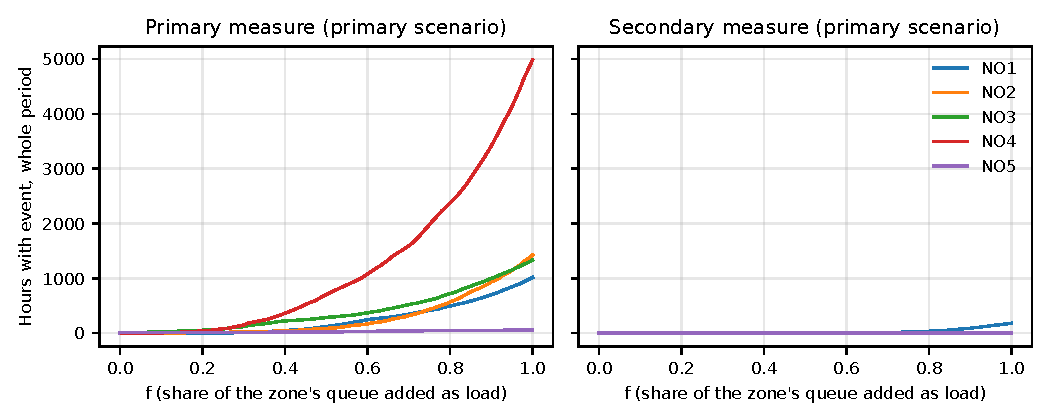
\includegraphics[width=\figbredde]{generert/fig_f_kurver.pdf}
\caption{Hours with an event over the whole period against $f$, per zone, primary scenario. Left: primary measure. Right: secondary measure (optimistic upper bound).}
\label{fig:f}
\end{figure}

\begin{table}[p]
\centering
\caption{Subperiods before and after the JAO MTU shift, primary scenario: valid MTUs, share of event MTUs and share of event hours (\%). The share of event MTUs is not pooled across the subperiods.}
\label{tab:delp}
\small
% generert av tools/lag_manus.py fra resultater/utfall.csv sha256 0b44f987e967e11133af9527bd3b88843689661e4add3e3314686f67ee287b13 [GT-647]
\begin{tabular}{llrrrrrr}
\toprule
Measure & Zone & \multicolumn{3}{c}{Before the MTU shift (60-min MTU)} & \multicolumn{3}{c}{After the MTU shift (15-min MTU)} \\
\cmidrule(lr){3-5}\cmidrule(lr){6-8}
 & & valid MTU & \% MTU & \% hours & valid MTU & \% MTU & \% hours \\
\midrule
\multicolumn{8}{l}{\emph{primary measure, primary scenario, $f = 0.50$}} \\
 & NO1 & 8062 & 0.30 & 0.30 & 38020 & 0.88 & 1.01 \\
 & NO2 & 8062 & 0.66 & 0.66 & 38020 & 0.27 & 0.34 \\
 & NO3 & 8062 & 2.42 & 2.42 & 38020 & 0.83 & 0.95 \\
 & NO4 & 8062 & 4.80 & 4.80 & 38020 & 2.95 & 3.31 \\
 & NO5 & 8062 & 0.22 & 0.22 & 38020 & 0.04 & 0.05 \\
\multicolumn{8}{l}{\emph{primary measure, primary scenario, $f = 1.00$}} \\
 & NO1 & 8062 & 7.11 & 7.11 & 38020 & 4.48 & 4.65 \\
 & NO2 & 8062 & 7.54 & 7.54 & 38020 & 7.44 & 8.58 \\
 & NO3 & 8062 & 7.39 & 7.39 & 38020 & 7.31 & 7.75 \\
 & NO4 & 8062 & 36.01 & 36.01 & 38020 & 20.62 & 21.89 \\
 & NO5 & 8062 & 0.38 & 0.38 & 38020 & 0.20 & 0.23 \\
\multicolumn{8}{l}{\emph{secondary measure, primary scenario, $f = 0.50$}} \\
 & NO1 & 8062 & 0.00 & 0.00 & 38020 & 0.00 & 0.00 \\
 & NO2 & 8062 & 0.00 & 0.00 & 34855 & 0.00 & 0.00 \\
 & NO3 & 8062 & 0.00 & 0.00 & 35479 & 0.00 & 0.00 \\
 & NO4 & 8062 & 0.00 & 0.00 & 38020 & 0.00 & 0.00 \\
 & NO5 & 8062 & 0.00 & 0.00 & 36913 & 0.00 & 0.00 \\
\multicolumn{8}{l}{\emph{secondary measure, primary scenario, $f = 1.00$}} \\
 & NO1 & 8062 & 0.41 & 0.41 & 38020 & 1.48 & 1.55 \\
 & NO2 & 8062 & 0.00 & 0.00 & 34855 & 0.00 & 0.00 \\
 & NO3 & 8062 & 0.00 & 0.00 & 35479 & 0.00 & 0.00 \\
 & NO4 & 8062 & 0.00 & 0.00 & 38020 & 0.00 & 0.00 \\
 & NO5 & 8062 & 0.00 & 0.00 & 36913 & 0.00 & 0.00 \\
\bottomrule
\end{tabular}

\end{table}

\begin{table}[p]
\centering
\caption{Sensitivities, run one at a time: hours with an event over the whole period. \emph{utilisation 1.0} replaces $b$ in both places; \emph{queue read 09.11} replaces $R$ and $Q$.} % GT-186 GT-316 GT-187
\label{tab:sens}
\small
% generert av tools/lag_manus.py fra resultater/utfall.csv sha256 0b44f987e967e11133af9527bd3b88843689661e4add3e3314686f67ee287b13 [GT-647]
\begin{tabular}{lllrrrrr}
\toprule
Measure & Scenario & Zone & \multicolumn{4}{c}{Hours with event, $f =$} & Valid hours \\
\cmidrule(lr){4-7}
 & & & 0.25 & 0.50 & 0.75 & 1.00 & \\
\midrule
primary & primary & NO1 & 3 & 120 & 418 & 1015 & 17567 \\
 &  & NO2 & 15 & 85 & 431 & 1424 & 17567 \\
 &  & NO3 & 77 & 285 & 603 & 1333 & 17567 \\
 &  & NO4 & 81 & 702 & 1979 & 4984 & 17567 \\
 &  & NO5 & 13 & 23 & 45 & 53 & 17567 \\
\addlinespace
 & utilisation 1.0 & NO1 & 31 & 378 & 1396 & 4530 & 17567 \\
 &  & NO2 & 31 & 353 & 1898 & 4482 & 17567 \\
 &  & NO3 & 179 & 541 & 1576 & 2955 & 17567 \\
 &  & NO4 & 265 & 1752 & 6507 & 12128 & 17567 \\
 &  & NO5 & 16 & 42 & 54 & 64 & 17567 \\
\addlinespace
 & queue read 09.11 & NO1 & 3 & 123 & 420 & 1040 & 17567 \\
 &  & NO2 & 18 & 132 & 698 & 2205 & 17567 \\
 &  & NO3 & 93 & 305 & 708 & 1540 & 17567 \\
 &  & NO4 & 80 & 697 & 1953 & 4910 & 17567 \\
 &  & NO5 & 13 & 23 & 45 & 53 & 17567 \\
\addlinespace
secondary & primary & NO1 & 0 & 0 & 18 & 180 & 17567 \\
 &  & NO2 & 0 & 0 & 0 & 0 & 16717 \\
 &  & NO3 & 0 & 0 & 0 & 0 & 16919 \\
 &  & NO4 & 0 & 0 & 0 & 0 & 17567 \\
 &  & NO5 & 0 & 0 & 0 & 0 & 17281 \\
\addlinespace
 & utilisation 1.0 & NO1 & 0 & 13 & 281 & 1715 & 17567 \\
 &  & NO2 & 0 & 0 & 0 & 0 & 16717 \\
 &  & NO3 & 0 & 0 & 0 & 4 & 16919 \\
 &  & NO4 & 0 & 0 & 0 & 0 & 17567 \\
 &  & NO5 & 0 & 0 & 0 & 0 & 17281 \\
\addlinespace
 & queue read 09.11 & NO1 & 0 & 0 & 19 & 184 & 17567 \\
 &  & NO2 & 0 & 0 & 0 & 0 & 16717 \\
 &  & NO3 & 0 & 0 & 0 & 0 & 16919 \\
 &  & NO4 & 0 & 0 & 0 & 0 & 17567 \\
 &  & NO5 & 0 & 0 & 0 & 0 & 17281 \\
\bottomrule
\end{tabular}

\end{table}

\begin{figure}[t]
\centering
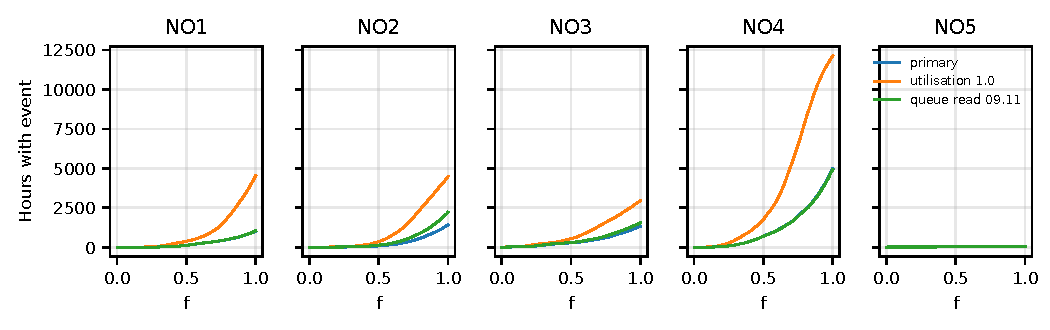
\includegraphics[width=\figbredde]{generert/fig_sensitivitet.pdf}
\caption{Primary measure: hours with an event against $f$ per zone for the primary scenario and the two sensitivities.}
\label{fig:sens}
\end{figure}

\begin{table}[t]
\centering
\caption{Missing MTUs and hours per zone and measure over the whole period, and MTUs with $H<0$ (primary measure).} % GT-375
\label{tab:mangl}
\footnotesize
% generert av tools/lag_manus.py fra resultater/manglende_per_maaned.csv sha256 edaf6454073df4e1e9c64f455c1522abbe721007e7b03ab41978d52e99841e97 [GT-649]; resultater/h_under_null.csv sha256 204cdbca68e3a99eea6e7e40649465cddd1e3c24253329a3f213942d1083d596 [GT-648]
\begin{tabular}{lrrrrrrr}
\toprule
Zone & MTU in grid & \multicolumn{2}{c}{Missing MTU} & Hours in grid & \multicolumn{2}{c}{Missing hours} & MTU with $H<0$ \\
\cmidrule(lr){3-4}\cmidrule(lr){6-7}
 & & primary & secondary & & primary & secondary & (primary) \\
\midrule
NO1 & 46086 & 4 & 4 & 17568 & 1 & 1 & 0 \\
NO2 & 46086 & 4 & 3169 & 17568 & 1 & 851 & 0 \\
NO3 & 46086 & 4 & 2545 & 17568 & 1 & 649 & 0 \\
NO4 & 46086 & 4 & 4 & 17568 & 1 & 1 & 0 \\
NO5 & 46086 & 4 & 1111 & 17568 & 1 & 287 & 8 \\
\bottomrule
\end{tabular}

\end{table}

The numbers are counts of MTUs and hours in which the added load would exceed the published headroom.
They are not estimates of unserved energy or of actual import needs.

\section{Limitations}
\label{sec:begr}

The limitations below are those of the preregistration, translated in full; the bullet on \texttt{netPos} is updated for deviation A2.
\begin{itemize}
\item The extremes are not simultaneously feasible: ``simultaneous feasibility of e.g. maximum flow on two borders cannot be guaranteed''~\cite{jaohb}. Each minimum net position is a separate extreme of the domain. The result is an optimistic upper bound for available import, given that the domain does not move. % GT-084 GT-083
\item The domain would move with large new load, and system properties, voltage and stability lie outside the method. Statnett gave system properties as the reason for the halt~\cite{press}, and § 14 of the Norwegian regulation on the system responsibility (fos) concerns approval of plant functionality~\cite{press}. % GT-193 GT-037 GT-038
\item Queues in other zones are left out. % GT-194
\item Queue figures vary with source and date: the press release gives 4~200 MW reserved and 9~100 MW in the queue~\cite{press}; the Power BI reading of 02.11 gives 4~190 and 10~109, which is the queue of the primary analysis~\cite{pbi}; the reading of 09.11 gives 4~205 and 10~774 and is not archived with a screenshot~\cite{pbi}; the long-term market analysis gives about 4200 and about 8800~\cite{lma}. % GT-040 GT-041 GT-185 GT-016 GT-017 GT-187 GT-045 GT-046 GT-120
\item Reserved and connected capacity: when a project is connected, its status changes from reserved to connected, but some connected projects with actual power exchange are still listed as reserved, because the cases are updated at least once a year~\cite{pbi}. Statnett's reserved figures can therefore include projects already connected, so the same capacity can be counted both in the net position and in the queue; events may then be overestimated, by an unknown amount. % GT-341 GT-342 GT-343 GT-370
\item The last year of the period uses $E_y$ for January--October, while 2024 and 2025 use full-year values from the v1 parameter file. % GT-180 GT-339 GT-200
\item The preregistration noted that \texttt{netPos} gave no data for the first delivery day; in the data run \texttt{netPos} had no data for 575 business days, and with deviation A2 the realised net position comes from \texttt{fbDomainShadowPrice}, which covers the whole period. % GT-165 GT-488 GT-572 GT-612
\item The secondary measure is an optimistic upper bound: outages are not subtracted. % GT-350
\end{itemize}

\section{Data and code availability}
\label{sec:tilgang}

No JAO raw data and no JAO time series are published. % GT-546 GT-190
The JAO terms define the Information Systems as ``any electronic system, application, database, website, API, or any other digital platform, including but not limited to the JAO Website, the IIP Website and all its subpages and related links, that are owned, operated, or controlled by JAO''~\cite{jaoterms}. % GT-744
Section A of the terms carries the heading ``GENERAL PROVISIONS APPLICABLE TO ALL USE OF THE INFORMATION SYSTEMS''~\cite{jaoterms}. % GT-745
Under the clause on access and use, ``When accessing the Information Systems and using the Content, a User shall'', among other things, ``mention the Information Systems as the source of the Content, in accordance with good industry practices''~\cite{jaoterms}. % GT-747 GT-748
The clause on restrictions on use has two provisions on passing content on~\cite{jaoterms}.
The first reads: ``The Content cannot be sold, commercialized as a product or service, marketed or otherwise made available to any third party, in whole or in part, in any manner, freely or against payment, unless expressly authorized in advance by JAO in writing''~\cite{jaoterms}. % GT-749 GT-061
The second reads: ``The Content cannot be disseminated, displayed, copied, extracted, distributed or reproduced in whole or in part, in any manner, on any medium or support whatsoever, freely or against payment, unless expressly authorized in advance by JAO in writing, or unless it is consistent with a Legitimate Use or otherwise permitted by these Terms of Use''~\cite{jaoterms}. % GT-750 GT-062
``Legitimate Use'' is defined as any of a list of uses, of which the first is ``Use for educational, academic or research purposes''~\cite{jaoterms}. % GT-746 GT-060
For the purposes of the restrictions, content includes ``materials derived from, based on, generated from or incorporating the Content''~\cite{jaoterms}. % GT-063
The outcome tables and figures in this manuscript are published with the JAO Nordic Publication Tool (\url{https://publicationtool.jao.eu}) as source (deviation A1). % GT-547 GT-748
Code, including the retrieval scripts, is published so that others can retrieve the data themselves; after the data run the scripts were given a fixed pause between calls and a wait after HTTP 429, whereas the data run itself used no pause. % GT-547 GT-477 GT-664
ENTSO-E and Elhub data are used under their own terms; the Elhub dataset is CC BY 4.0~\cite{elhub}. % GT-675
All sources are listed in the supplement \texttt{sources.csv}~\cite{sources}.

\section{Use of AI tools}
\label{sec:ki}

The analysis was planned and carried out with Claude Code as a tool under the author's direction.
Tools and models, read from the session logs: Claude Code 2.1.317, main session on \texttt{claude-opus-5-5}; \texttt{claude-sonnet-5-5} gave 17 of the main session's answers, all in the interval 2026-11-09T16:27:15.690Z to 2026-11-09T16:27:46.448Z. % GT-668 GT-669 GT-398
Subagents in Claude Code, all on \texttt{claude-opus-5-5}: 4 for source reading, 23 for blind verification of ground-truth rows, 4 for independent review of the preregistration, and 2 for the independent recomputation of the outcomes; 33 in all, counted when this manuscript was written (later subagents are recorded in the repository). % GT-671 GT-672 GT-673 GT-674 GT-670
Chat-Claude (claude.ai) was used for the author's own review; according to the author, it ran Claude Opus 5.5 (\texttt{claude-opus-5-5}) throughout, without a change of model; this is the author's statement, archived as source K-115 in \texttt{sources.csv}~\cite{sources}, not a reading of the session logs. % GT-678 GT-401
``The author made the methodological choices, had every figure checked against its source, and is responsible for the content.'' % GT-191

\begin{thebibliography}{99}
\raggedright
\bibitem{press} Statnett SF. \emph{Midlertidige tiltak for fortsatt forsvarlig systemdrift} [Temporary measures for continued secure system operation]. Press release, published 09.11.2026 08:45. \url{https://www.statnett.no/om-statnett/nyheter-og-pressemeldinger/nyhetsarkiv-2026/midlertidige-tiltak-for-fortsatt-forsvarlig-systemdrift/}. Read 2026-11-09. % GT-681 GT-680 GT-705 GT-693
\bibitem{pbi} Statnett SF. Data-centre connection cases and reservations, Power BI dashboard. \url{https://www.statnett.no/nettkapasitet-til-produksjon-og-forbruk/foresporsler-og-reservasjon-i-nettet/}. Read 02.11.2026 and 09.11.2026; definitions read 2026-11-09. % GT-712 GT-185 GT-187 GT-180 GT-702
\bibitem{statnettbrev} Statnett SF. \emph{Svar på brev -- NVE ber om informasjon om utredninger av forsyningssikkerhet i Nord-Norge} [Reply to NVE on security of supply in Northern Norway]. Letter, 15 June 2026. \url{https://www.statnett.no/globalassets/for-aktorer-i-kraftsystemet/nyheter-for-aktorer-i-kraftbransjen/svarbrev-nve-om-utredninger-av-forsyningssikkerhet-i-nord-norge-15-06-2026.pdf}. Read 2026-11-09. % GT-689 GT-688 GT-711 GT-694
\bibitem{lma} Statnett SF. \emph{Langsiktig markedsanalyse 2026-60} [Long-term market analysis]. October 2026. \url{https://www.statnett.no/globalassets/for-aktorer-i-kraftsystemet/planer-og-analyser/lma/langsiktig-markedsanalyse_2026-2060.pdf}. Read 2026-11-09. % GT-313 GT-687 GT-710 GT-692
\bibitem{jaohb} JAO S.A. \emph{Nordic Publication Tool Handbook}, Version 1.8.1, 02-07-2026. \url{https://publicationtool.jao.eu/PublicationHandbook/Nordic_PublicationTool_Handbook_v1.8.1.pdf}. Read 2026-11-09. % GT-081 GT-707 GT-697
\bibitem{jaoterms} JAO S.A. \emph{General Terms and Conditions for the use of the Information Systems}. \url{https://www.jao.eu/terms-conditions}. Read 2026-11-09. % GT-706 GT-695
\bibitem{jaopy} F. Boerman-Lima. \emph{jao-py}, version 0.8.7. \url{https://github.com/fboerman/jao-py}. Read 2026-11-09. % GT-691 GT-055 GT-690 GT-698
\bibitem{ccm2020} Nordic CCR TSOs. \emph{Nordic Capacity Calculation Region capacity calculation methodology}, approved text. 14 October 2020. \url{https://nordic-rcc.net/wp-content/uploads/2024/01/CACM-Nordic-CCR-DA-and-ID-CCM-2020-1.pdf}. Read 2026-11-09. % GT-685 GT-708 GT-700 GT-686
\bibitem{ccm2026} Nordic CCR TSOs. \emph{Nordic Capacity Calculation Region capacity calculation methodology}, amendment, legal proposal. 19 May 2026. \url{https://nordic-rcc.net/wp-content/uploads/2026/10/CCM-legal-proposal-RfA-2026__clean_Vf.pdf}. Read 2026-11-09. % GT-686 GT-709 GT-701
\bibitem{xu} A. L. Xu and C. Stiewe. \emph{Competitive effects of transmission constraints in the German electricity market}. arXiv:2607.00977v1 [econ.GN], 1 Jul 2026. Read 2026-11-09. % GT-682 GT-683 GT-071 GT-684 GT-696
\bibitem{entsoe} ENTSO-E. \emph{Transparency Platform}: installed capacity per production type (A68), actual generation per production type (A75) and cross-border physical flows (A11). \url{https://transparency.entsoe.eu/}. Retrieval times in Section~\ref{sec:data}; platform read 2026-11-09. % GT-699
\bibitem{elhub} Elhub. \emph{consumption\_datacenter\_per\_mba\_hour}, CC BY 4.0. Downloaded 2026-11-02; the file used is the one distributed with KHEPRI-DC v1~\cite{v1}. % GT-675
\bibitem{v1} E. Botten Nicolaysen. \emph{KHEPRI-DC v1.0.0: Timevis nettoposisjon per norsk budområde 2023--2025 med datasenterkøen lagt på}. Zenodo, version 1.0.0, doi:10.5281/zenodo.23887356 (version DOI). The files were read from git tag v1.0.1, whose content is identical to this deposit. Concept DOI: doi:10.5281/zenodo.23887355. Metadata read 2026-11-09. % GT-005 GT-006 GT-004 GT-002 GT-247 GT-704
\bibitem{osf} E. Botten Nicolaysen. \emph{KHEPRI-DC-FB: preregistration v1}. OSF Registries, submitted 2026-11-09 with an embargo until 31.12.2027 selected. \url{https://osf.io/vd9np}. % GT-437 GT-438 GT-753
\bibitem{sources} Supplement \texttt{sources.csv}: all archived sources with title, publisher, URL, retrieval time (UTC) and sha256, generated from the repository's source manifest.
\end{thebibliography}

\end{document}
